\chapter{$\Na/\Ca$ Exchanger}
\label{chap:NCX}

\def\NaCa{{\text{NaCa}}}

\section{Introduction}

$\Na/\Ca$ exchanger (NCX) is the major mechanism for extruding calcium out of
myoplasm of cardiac myocytes via sarcolemma. Of the total calcium involved in
contraction ($I_\LCC$ + SR $\Ca$ release), 90\% is taked up by the SERCA pumps
and the rest (typically the calcium influx via LCC) is extruded by NCX
\citep{bers2002ncx}.  NCX is also found to affect level of $\Ca$ in the SR at
rest \citep{blaustein1999}. Thus, it has been suggested that NCX may play a
significant role in cardiac arrhythmia, in which NCX trigger spontaneous $\Ca$
release and spontaneous AP.



\subsection{stoichiometry}
\label{sec:NCX-stoichiometry}

The stoichiometry for $\Ca$ transport is three $\Na$ ions exchanged for one
$\Ca$ ion (i.e. 3Na:1Ca) \citep{reeves1984}. Some workers have raised the
possibility of 4: 1 on theoretical ground (Sect.\ref{sec:ncx-mullins-1977}) and
experimentally in dog heart vesicles (Ledvora \& Hegyvary, 1983); yet 3:1 was
more widely accepted.

The ATP-driven pumps, e.g. PMCA, have high affinity to $\Ca$, yet very
low turnover rates, i.e. number of $\Ca$ transported per carrier per
unit of time, i.e. 100s$^{-1}$
(Chap.~\ref{chap:PMCA})~\citep{blaustein1999}.
\textcolor{red}{$\NaCa$ exchanger are non-ATP driven, with 10-fold lower
  affinity, yet 10- to 50-fold higher turnover rate}. The high
turnover rate is important, to extrude quickly $\Ca$ at high
$[\Ca]_i$. 

\begin{framed}
  A single open $\Ca$ channel has a turnover rate of up to $10^7$
  ions/s~\citep{hille1992mb}, a single exchanger can transport up to
  $\sim 5\times 10^3$ $\Ca$/s, and a PMCA or SERCA pump or $\NaCa$ pump
  can transport $\sim 10^2$ $\Ca$/s~\citep{stein1986}.
\end{framed}

\subsection{E\_NaCa: reversial potential of NCX}
\label{sec:NCX-reversial-potential}

In general (Na:Ca ratio = n:1), the reversial potential is expressed as
\begin{equation}
E_\NaCa = (n E_\na - 2 E_\ca) / (n-2)
\end{equation}

In 3:1 Na:Ca ratio, the reversal potential of NCX ($E_\text{Naca}$) is
\begin{equation}
E_\NaCa = 3 E_\na - 2 E_\ca
\end{equation}

In the condition of 140 mM $[\Na]_o$; 30 mM $[\Na]_i$; 1 mM $[\Ca]_o$; 73 nM
$[\Ca]_i$; then $E_\NaCa = -131$ mV.

In the condition of 140 mM $[\Na]_o$; 20 mM $[\Na]_i$; 67 nM
$[\Ca]_i$; then 
\begin{itemize}
  
  \item 0.1 mM $[\Ca]_o$: $E_\NaCa = -39$ mV.
  
  \item 1 mM $[\Ca]_o$: $E_\NaCa = -100$ mV.
  
  \item 2 mM $[\Ca]_o$: $E_\NaCa = -119$ mV.
\end{itemize}

The I-V curve under 0.1mM $[\Ca]_o$ (control, trace (a)) and 1mM $[\Ca]_o$
(trace (b)) cross at the very negative potential range. The peak I was chosen as
the early stage of the peak shift of holding current. 

To avoid the background current, subtracting trace (a) from trace (b) can reveal
the carrier-mediated Na-Ca exchange curent. It shows an exponential growth I-V shape, i.e.
exponential voltage-dependency, which is revealed by a semi-logarithmic plot
(Kimura et al., 1987) - Sect.\ref{sec:NCX_Kimura_1987}.





\subsection{forward mode and reverse mode}
\label{sec:NCX-forward-mode}
\label{sec:NCX-reverse-mode}

$\NaCa$ exchangers have been found to work in 2 modes: ``$\Ca$ exit
mode'' (forward mode) and ``$\Ca$ entry mode'' (reverse mode). 

NCX can display either inward current or outward currents depending upon the
concentration of $\Ca$ and $\Na$; each direction is mediated by the ion in
different sides of the membrane

\begin{itemize}

\item The forward mode (inward $I_\ncx$) is favoured by high $[\Ca]_i$, low
$[\Na]_i$ and polarized membrane potential.

Here: $\Na$ in and calcium efflux. The inward component shows a sigmoidal
dependency of $[\Na]_o$ with $K_i = 87.5\pm 10.7$ mM; and Hill coefficient of
2.9$\pm$0.4. 

\item The reverse mode (outward $I_\ncx$) is favored by the opposite
\textcolor{red}{NCX current is outward current with low $[\Ca]_i$ (i.e. resting
state, 1 $\Ca$ in - 3 $\Na$ out) which is positive value}

It shows a sigmoidal dependence upon $[\Ca]_o$ with half-maximum concentration
$K_i = 1.38$ mM; with Hill coefficient 0.9$\pm$0.2.

If we replace $\Ca$ with $\ce{Sr^2+}$, then $K_i=7$ mM. NCX is not activated by
$\Mg$ and $\Ba$. 

\end{itemize}


So, the direction of $I_\ncx$ is determined by electrochemical
potential.  So, the total current is the subtraction of the two components
(Sect.\ref{sec:NCX_Kimura_1987})
\begin{equation}
\begin{split}
I_{\ncx,in} = ([\Na]_i)^m [\Ca]_o \exp\left( (n-2) . r . F.\Vm/(RT) \right) \\
I_{\ncx,out} = ([\Na]_o)^m [\Ca]_i \exp\left( -(n-2).(1-r) F.\Vm/(RT) \right) \\
I_{\ncx} = k \times (I_{\ncx,in} - I_{\ncx,out})
\end{split}
\end{equation}
with $k$ is scaling factor; $m$ is Hill coefficient for sodium.
\textcolor{red}{Based on the Hill coefficients determined above}, we use 3 for
sodium; and 1 for calcium.

If we assume that $k$ is constant, then the difference-current at two values of
external $[\Ca]_o$ is
\begin{equation}
i_{\text{diff},\ncx} = k ([\Na]_i)^n (\text{1mM $[\Ca]_o$} - \text{0.1mM
$[\Ca]_o$}) \times \exp\left( r.F.\Vm/(RT)\right)
\end{equation}
By fitting it with the subtracted curve (Fig. 3B Kimura et al., 1987), then 
$k = 2.07 \times 10^{-5} \muA/\text{mM}^4.\muF$; and $r=0.38$.



\subsection{allosteric regulation}
\label{sec:NCX-allosteric-regulation}

It's also believed that NCX is allosterically regulated by $[\Ca]_i$ such that
low $[\Ca]_i$ can deactivate $I_\ncx$~\citep{miura1989}
(Sect.\ref{sec:weber-et-al}).
Recently,~\citep{urbanczyk2006} pointed out that allosteric coupling is not
required at high $[\Na]_i$.


\subsection{I-V curve}
\label{sec:I-V-curve-NCX}

The I-V curve is explained in Sect.\ref{sec:I-V-curve}. The I-V curve for NCX
was investigated near the reversal potential. The reversal potential of NCX is
given by
\begin{equation}
E_\NCX = (n E_\na - z_\ca E_\ca) / (n-z_\ca)
\end{equation}
with $n$ = (the stoichiometry for $\Na$) the number of $\Na$ ions in exchanged
for one $\Ca$ ion, $z_\ca=2$ is the valence of $\Ca$ ion.

Suppose the stoichiometry is 3:1 then
\begin{equation}
E_\NCX = (3 E_\na - z_\ca E_\ca) 
\end{equation}


\subsection{-- Erev of NCX}
\label{sec:equilibrium-ncx}


At resting condition, extracellular $\Na$ and $\Ca$ are usually high,
450mM and 3-4mM in marine vertebrates~\citep{blaustein1974},
respectively, and 120-145mM and 3-4mM in other vertebrates (the
dominant). Sect.\ref{sec:ion-concentration-neuron}

Under ionic conditions closed to physiological ones: 140 mM-external Na+, 20
mM-internal Na+, 67 nM-internal Ca2+, the values of $E_\NCX$ at 1 mM- and 2mM-
external Ca2+ are -100 mV and -119 mV respectively.

The intracellular concentrations of $\Na$ and $\Ca$ are relatively low, 10mM and
0.1$\mu$M, respectively. So, there is a high, inward electrochemical gradient of
both ions.

At the negative potential $V_m$ on the order of -80 or -60
mV~\citep{blaustein1999}, the energetic and kinetics exchange are
described as follows
\begin{itemize}
\item The large inwardly electrochemical gradient for sodium is defined as
  \begin{equation}
    \label{eq:1168}
    \begin{split}
      \Delta\overline{\mu}_\na &= z_\na F(E_\na-V_m)  \\
      &= RT\ln\left(\frac{[\Na]_o}{[\Na]_i}\right) - z_\na V_mF
    \end{split}
  \end{equation}
based on Nernst equation (Sect.\ref{sec:nernst-equation}). 

\item The very large, inwardly electrochemical gradient for calcium is
  defined as
  \begin{equation}
    \label{eq:1169}
    \begin{split}
      \Delta\overline{\mu}_\ca &= z_\ca F(E_\ca-V_m)  \\
      &= RT\ln\left(\frac{[\ca]_o}{[\ca]_i}\right) - z_\ca F V_m
    \end{split}
  \end{equation}

\end{itemize}

The kinetics of $\NaCa$ exchanger must conform to the assumption that
the sole source of energy is the $\Na$ gradient. So, if the coupling
ratio $\NaCa$ is $n$, then at equilibrium we have
$n\Delta\overline{\mu}_{\na} = \Delta\overline{\mu}_{\ca}$ via the carrier.

\begin{framed}
  In the case of $\NaCa$ plus K exchanger, the fluxes of $\Ca$ is coupled
  with one $\K$ to counterflow $r$ $\Na$ ions, then
  \begin{equation}
    \label{eq:1170}
    r\Delta\overline{\mu}_{\na} = \Delta\overline{\mu}_{\ca} + \Delta\overline{\mu}_\k
  \end{equation}
  with $ \Delta\overline{\mu}_\k = z_\k F(E_\k-V_m) $.
\end{framed}


{\bf $\NaCa$ exchanger}: At equilibrium, we have
\begin{equation}
  \label{eq:1162}
  n z_\na F(E_\na-V_m) = z_\ca F(E_\ca-V_m)  
\end{equation}
or
\begin{equation}
  \label{eq:1173}
  n \left(\ln\left(\frac{[\Na]_o}{[\Na]_i}\right) - \frac{z_\na
      V_mF}{RT}\right) = 
  \ln\left(\frac{[\ca]_o}{[\ca]_i}\right) - \frac{z_\ca V_mF}{RT}
\end{equation}
then take the exponential on both side
\begin{equation}
  \label{eq:1172}
  \frac{\left(\frac{[\na]_o}{[\na]_i}\right)^n}{\exp\left(\frac{nz_\na
        V_mF}{RT}\right)} =   \frac{\frac{[\ca]_o}{[\ca]_i}}{\exp\left(\frac{z_\ca
        V_mF}{RT}\right)}
\end{equation}
 or
\begin{equation}
  \label{eq:1171}
  \begin{split}
    \frac{[\Ca]_o}{[\Ca]_i} &= \left(\frac{[\na]_o}{[\na]_i}\right)^n 
    \exp\left( -(nz_\na-z_\ca)\frac{V_mF}{RT} \right) \\
    &=\left(\frac{[\na]_o}{[\na]_i}\right)^n 
    \exp\left( -(n-2)\frac{V_mF}{RT} \right) 
  \end{split}
\end{equation}

\begin{framed}
  In the case of $\NaCa$ plus K exchanger, the expansion for the
  equation is
  \begin{equation}
    \label{eq:1174}
    \begin{split}
      \frac{[\Ca]_o}{[\Ca]_i} &= \left(\frac{[\na]_o}{[\na]_i}\right)^n 
      \left(\frac{[\k]_o}{[\k]_i}\right)
      \exp\left( -(nz_\na-z_\ca-z_\k)\frac{V_mF}{RT} \right)    \\
      &= \left(\frac{[\na]_o}{[\na]_i}\right)^n 
      \left(\frac{[\k]_o}{[\k]_i}\right)
      \exp\left( -(n-3)\frac{V_mF}{RT} \right)    
    \end{split}
  \end{equation}
\end{framed}

\subsection{coupling ratio vs. stoichiometry}

\textcolor{red}{Let's make clear 2 concepts: $n$ is called the
  coupling ratio, also denoted as $n_T$ using Lauger
  terminology~\citep{lauger1991}. This may be of different value from
  the number of binding sites for $\Na$ and $\Ca$ on the exchanger,
  known as stoichiometry $n_B$}
(Sect.~\ref{sec:binding-sites}).  

It's very hard to measure $n_B$ and $n_T$. The ratio of $[\Ca]_i$-dependent
$\Na$ influx, to the $[\Na]_o$-dependent $\Ca$ efflux is
3.1:1~\citep{blaustein1975}. However, most of the data agree with the ration
n=3:1. Exchange is therefore a rheogenic (current-generating) process.

% If $n=n_T=3$, then eq.~\eqref{eq:1171} is simplified as
% \begin{equation}
%   \label{eq:1460}
%   \frac{[\Ca]_o}{[\Ca]_i} =\left(\frac{[\na]_o}{[\na]_i}\right)^n 
%   \exp\left( -\frac{V_mF}{RT} \right)   
% \end{equation}

In a detail review by~\citep{blaustein1999}, it was shown that the
$\NaCa$ exchanger in cardiac/neuronal tissue (but not ROS)
\begin{itemize}
\item does not normally transport other ions along with the $\Na$ and $\Ca$
\item likely has the coupling ratio $n=3:1$
\end{itemize}
Thus, a proper form for the eq.~\eqref{eq:1171} is
\begin{equation}
  \label{eq:1175}
  \frac{[\Ca]_o}{[\Ca]_i} = \left(\frac{[\na]_o}{[\na]_i}\right)^3
  \exp\left( -\frac{V_mF}{RT} \right)
\end{equation}

\subsection{stoichiometry}

The ratio of $\Na$ and $\Ca$ exchange is a topic of debated
\begin{itemize}
  \item 3 Na in / 1 Ca out: ~\citep{reeves1984,kimura1987} 
  
  \item 4 Na in / 1 Ca out: ~\citep{mullins1979, mullins1991, fukioka2000}
  
  \item 2 Na in / 1 Ca out: ~\citep{niedergerke1963} 
\end{itemize}

Depending on the ratio, it can generate an inward current, or in early days,
with Na:Ca=2:1 ratio, NCX is considered as electrically neutral - the reason
why so it had not been incorporated into cellular models.
Later observation show that this ratio is larger than 2~\citep{blaustein1974}.
Nowadays, we know that it's not neutral. However, the ratio is not unique.
% where the influx of 3 $\Na$ is in exchanged for the efflux of 1 $\Ca$ ion,
% generating an inward current.

\begin{mdframed}


On cardiac cells~\citep{pitts1979, reeves1980, reeves1984, 
kimura1987,ehara1989}, squid axon~\citep{dipolo1990}, and barnacle muscle
cells~\citep{rasgado-flores1987, rasgado-flores1989}, the ratio is 3Na:1Ca.

Some other studies found $\K$ also involve in the process in vertebrate
photoreceptor exchanger with 4Na:1Ca+1K~\citep{dipoli1984, cervetto1989,
yasui1990}; or 4Na:1Ca~\citep{fukioka2000}. These $\K$-dependent exchanger and
$\K$-independent exchanger were found to co-expressed in rat
brain~\citep{tsoi1998}.  This may put a question to our current understanding of
the physiological role of NCX.

\end{mdframed}


\subsection{4 Modes of activity}
\label{sec:4-modes-activity}

In NCX, 3 $\Na$ in exchange for 1 $\Ca$ ion out. The activity of this pump use
the gradient of $\Na$, not ATP energy. So under reversal potential of the
exchanger, the exchanger operate in forward mode, with an inward current is
generated.
When the potential positive to the reversal potential (i.e. intracellular
$[\Na]_i$ is high enough), NCX operates in an opposite direction, producing a
calcium entry and generating an outward current.

\begin{enumerate}
\item forward mode: $\Ca$ exit mode, which is associated with an
  inward current and is thus augmented by a depolarization, and
  attenuated by a repolarization. 
\item reverse mode: $\Ca$ entry mode, which is associated with an
  efflux current and is thus augmented by a repolarization
\item $\Ca/\Ca$ exchange mode: mediated by NCX with the coupling ratio
  is 1:1~\citep{blaustein1975}, and is
  $V_m$-sensitive~\citep{dipolo1990}, though electroneutral.
\item $\Na/\Na$ exchange mode: mediated by NCX
\end{enumerate}

The kinetics of NCX in different species can be different. Some of the
kinetics parameters are modulated (indirectly) by ATP, and $V_m$ or
some other factors. The quantity we use is $K_{0.5}$ which is the
ionic concentration required at half-maximal activation or inhibition
of NCX.

\subsection{-- $\Ca$ entry mode}
\label{sec:calcium-entry-mode}

This mode is activated at site N1$_o$ by non-transported external
alkali metal ions, including $\Na$ ($\Khalf = 50-75$mM in squid
axons/crab nerve, $\Khalf = 2$mM in synaptosomes). Monovalents cations
but not alkali cannot activate, probably they cannot bind to
N1$_o$. However, high $[\Na]_o$ inhibit this mode ($\Khalf =
100-200$mM in squid axon, $\Khalf = 45-70$mM in mammalian
tissues). This inhibition is estimated to be a function of
$([\Na]_o)^2$, which means to inhibit the exchange, 2$\Na$ need to act
cooperatively.

\begin{framed}
  The biphasic of $[\Na]_o$ (activating and inhibiting) imply a
  complex kinetics. At low concentration, a single $\Na$ binds to site
  N1$_o$ and activate the $\Ca$ influx. At high concentration, a
  second $\Na$ binds to the second site N2$_o$, which may trigger a
  conformation changes that inhibit the binding of $\Ca$ to C2$_o$.
\end{framed}

The amount of $\Ca$ influx is a hyperbolic function of $[\Ca]_o$ ; and
a sigmoid function of $[\Na]_i$ with Hill coefficient of 3, i.e. $\Ca$
efflux is the result of cooperative action of at least 3$\Na$.
\begin{enumerate}
\item site C2$_o$: for $[\Ca]_o$
  \begin{itemize}
  \item in marine vertebrates: $\Khalf=50-100$mM (in $\Na$-containing
    media). In $\Na$-free media, the affinity is higher $\Khalf=2-7$mM.
  \item in mammalian heart, brain:  $\Khalf = 0.1-0.3$mM (much higher
    compared to marine vertebrates)
  \end{itemize}

\item site C1$_o$: no evidence of activation by $[\Ca]_o$. So, we
  don't care this site.

\item site C1$_i$: for $[\Ca]_i$
  \begin{itemize}
  \item in ATP-fueled cells: $\Khalf = 0.6-2\mu$M
  \item in ATP-depleted cells: $\Khalf$ is reduced by $\sim$ 10x. 
  \end{itemize}
  So, the binding affinity to site C1$_i$ is modulated by
  phosphorylation. 

  At low $[\Ca]_i< 0.01\mu$M, there is no $[\Ca]_o$-dependent $\Na$
  efflux or $\Na$-dependent influx is observed.

\item site N2$_i$: for $[\Na]_i$
  \begin{itemize}
  \item in mammalian cardiac muscle: $\Khalf = 15-25$mM
  \item in squid axon and barnacle muscle fibre: $\Khalf = 30-60$mM
  \end{itemize}
\end{enumerate}

When $[\Ca]_i$ increase, NCX would shift to $\Ca$ efflux mode, or
$\Ca/\Ca$ exchange mode. However, we don't know the mechanism yet.
Inhibition of $\Ca$ entry due to high $[\Na]_i$ (of 140mM), NCX would
shift to $\Ca$ efflux mode or $\Na/\Na$ exchange mode.

\subsection{-- $\Ca$ exit mode}
\label{sec:calcium-exit-mode}

The $\Ca$ efflux current is a function of $[\Ca]_i$;  and a sigmoid
function of $[\Na]_o$ of Hill coefficient of $\sim 3$.

\begin{enumerate}
\item activated by high internal $[\Ca]_i$
  \begin{itemize}
  \item in ATP-fueled cells: $\Khalf = 0.6-6\mu$M for both mammalian
    and marine vertebrates.
  \item in ATP-depleted cells: $\Khalf = 8-15\mu$M for squid axons
  \end{itemize}
  With 2 $\Ca$ binding sites, the one of lower affinity serves as
  transported site and the one with higher affinity C1$_i$ serves as
  catalytic role. When C1$_i$ is mutated, the affinity for C2$_i$ is
  greatly reduced. So, both sites cooperatively act to transport $\Ca$
  out.
\item for $[\Na]_o$
  \begin{itemize}
  \item in ATP-fueled squid axons: $\Khalf = 50-80$ mM
  \item in ATP-depleted squid axons: $\Khalf = 110-140$ mM
  \end{itemize}
The nature of the binding sites for $\Na$ at extracellular side is
unclear. ~\citep{blaustein1999} suggested one $\Na$ bind to N1$_o$
first, and then 2 other $\Na$ bind to N2$_o$. When all 3 are bound,
NCX starts to cycle. 
\end{enumerate}

It's suggested that N2$_i$ and C2$_i$ are the same site, just
different conformation. So, when $\Na$ bind to it, it block the $\Ca$
transport site and thus inhibiting $\Ca$ exit mode. On the other hand,
$[\Na]_i$ has no effect of inhibiting on $\Ca$ entry mode, but to
facilitate it.



\subsection{-- $\Ca/\Ca$ exchange mode}
\label{sec:caca-exchange-mode}

\begin{itemize}
\item for $[\Ca]_o$
  \begin{itemize}
  \item in squid axon and giant barnacle muscle fibers: $\Khalf = 1-3$mM
  \item in mammalian preparation: $\Khalf = 0.2-0.8$mM 
  \end{itemize}
\item for $[\Ca]_i$
  \begin{itemize}
  \item in ATP-fueled cells: $\Khalf \sim 2.5\mu$M for squid axons.
  \item in ATP-depleted cells: $\Khalf = 10-15\mu$M for squid axons
  \end{itemize}
\end{itemize}

The $V_m$-sensitive of this process impose that one of the
$\Ca$-binding stage is rate limiting, which is most likely related to
$\Khalf$ of $[\Ca]_i$.

\subsection{-- $\Na/\Na$ exchange mode}
\label{sec:nana-exchange-mode}

\begin{itemize}
\item for $[\Na]_o$
  \begin{itemize}
  \item from 120-130mM
  \end{itemize}
\item for $[\Na]_i$
  \begin{itemize}
  \item not yet been determined, but estimated to be in the order of
    10-20mM, as the saturated $[\Na]_i=100$mM. 
  \end{itemize}
\end{itemize}


\subsection{Kinetics exchange}
\label{sec:kinetics-exchange}


The net flux of $\Ca$ via NCX is governed by the difference between
$V_m$ and the reversal potential of the exchanger $E_\NCX$ and a rate
of exchange $k_\ncx$.
\begin{equation}
  \label{eq:1461}
  J_{\ca,\ncx} = k_\ncx (V_m-E_\ncx)
\end{equation}
with
\begin{equation}
  \label{eq:1462}
  E_\ncx=n_TE_\Na-2E_\ca
\end{equation}
where the reversal potential (or equilibrium potential) of each ion
species are based on Nernst equation
\begin{equation}
  \label{eq:1463}
  \begin{split}
    E_\na = \frac{RT}{z_\na F}\ln\frac{[\Na]_o}{[\Na]_i}\\
    E_\ca = \frac{RT}{z_\ca F}\ln\frac{[\Ca]_o}{[\Ca]_i}\\
  \end{split}
\end{equation}
For $\Na$, its net flux has an opposite direction
\begin{equation}
  \label{eq:1464}
  J_{\na,\ncx} = -n_T J_{\ca,\ncx}
\end{equation}
The variable $k_\ncx$ is a nonlinear, complex kinetic parameters that
is analogous to conductance density, i.e. conductance per unit area,
in ion channels. $k_\ncx$ depends upon
\begin{enumerate}
\item number of carriers, i.e. amount of NCX
\item fractional saturation of the carrier binding sites by the
  activating ions and transported ions
\item $V_m$
\item ATP (though may not direct, but it provides energy for the
  phosphorylation of the exchange, which alter the kinetics of
  bindings and translocation of transport ions)
\item other factors, e.g. phosphorylation and desphoshphorylation. 
\end{enumerate}
Under normal physiological condition, NCX appears to be at least
partially phosphorylated; which cause NCX exhibits a high affinity to
$[\Na]_o$ and $[\Ca]_i$~\citep{blaustein1977,dipoli1987}. So, there is
no $[\Na]_i$-dependent. The half-maximal activation of NCX in the
physiological range of $[\Ca]_i$ (from 0.1-1$\mu$M in squid axon,
barnacle muscle and cardiac muscle) plays an important role in the
physiological activity of NCX.

As ionic flow across NCX is rheogenic, we can write a current equation
equivalent to the flux equation to describe the net current density
$I_\ncx$ ($\mu$A/cm$^2$)
\begin{equation}
  \label{eq:1465}
  I_\ncx = g_\ncx (V_m-E_\ncx)
\end{equation}
NOTE: $I_\ncx = (J_{\na,\ncx}+J_{\ca,\ncx})\times dt$; and $g_\ncx$ is
the conductance per unit area (conductance density)

\begin{framed}
  In NCX, the $\Ca$ movement is outward if
  \begin{equation}
    \label{eq:1457}
    nz_\na F(E_\na-V_m) > z_\ca F(E_\ca-V_m)
  \end{equation}
  with $n$ is the coupling ratio Na:Ca. And it moves inward
  otherwise. See Sect.~\ref{sec:kinetics-exchange}.
\end{framed}


\subsection{Binding sites}
\label{sec:binding-sites}

There are several ion binding sites on NCX; some allows bound ion to
be transported; the others serve as activating role and are not
transported. There are two binding sites for $\Ca$ and two for $\Na$,
on each side
\begin{enumerate}
\item C1$_i$ = bind 1Ca (catalysis), C2$_i$ = bind 1 Ca (transport)
\item C1$_o$ = do something else, C2$_o$ = bind 1Ca (transport)
\item N1$_i$ = can bind 1 ion (either Na, K, Li) (catalysis or
  transport Na??), N2$_i$ = bind 2 (or 3) Na (transport)
\item N1$_o$ = can bind 1 ion (either Na, K, Li, Rb, Cs) (catalysis or
  transport Na??), N2$_o$ = bind 2 (or 3) Na (transport)
\end{enumerate}
RB and Cs have only been tested with N1$_o$, not with N1$_i$. In
addition, there is no evidence that there is a separate binding site
for the third $\Na$. So, may be the N1 sites serve as transport for
the 3Na; or the third one is transported in another
site. ~\citep{blaustein1999} speculated that the third one is
transported in N2, when the first 2 are bound to N1. 



\section{NCX: Mullins (1977)}
\label{sec:ncx-mullins-1977}

~\citep{mullins1977mnc} proposed a model for the Na/Ca exchangers.
This models assumed 4:1 coupling ratio, i.e. 4Na binding on one side before 1Ca
can bind on the other side. The 7-step sequential binding model is given in
Fig.~\ref{fig:Mullins_NaCa}. This choice is dictated by the energy
considerations and by the sensitivity of $\Ca$ fluxes to membrane potential.

\begin{figure}[hbt]
  \centerline{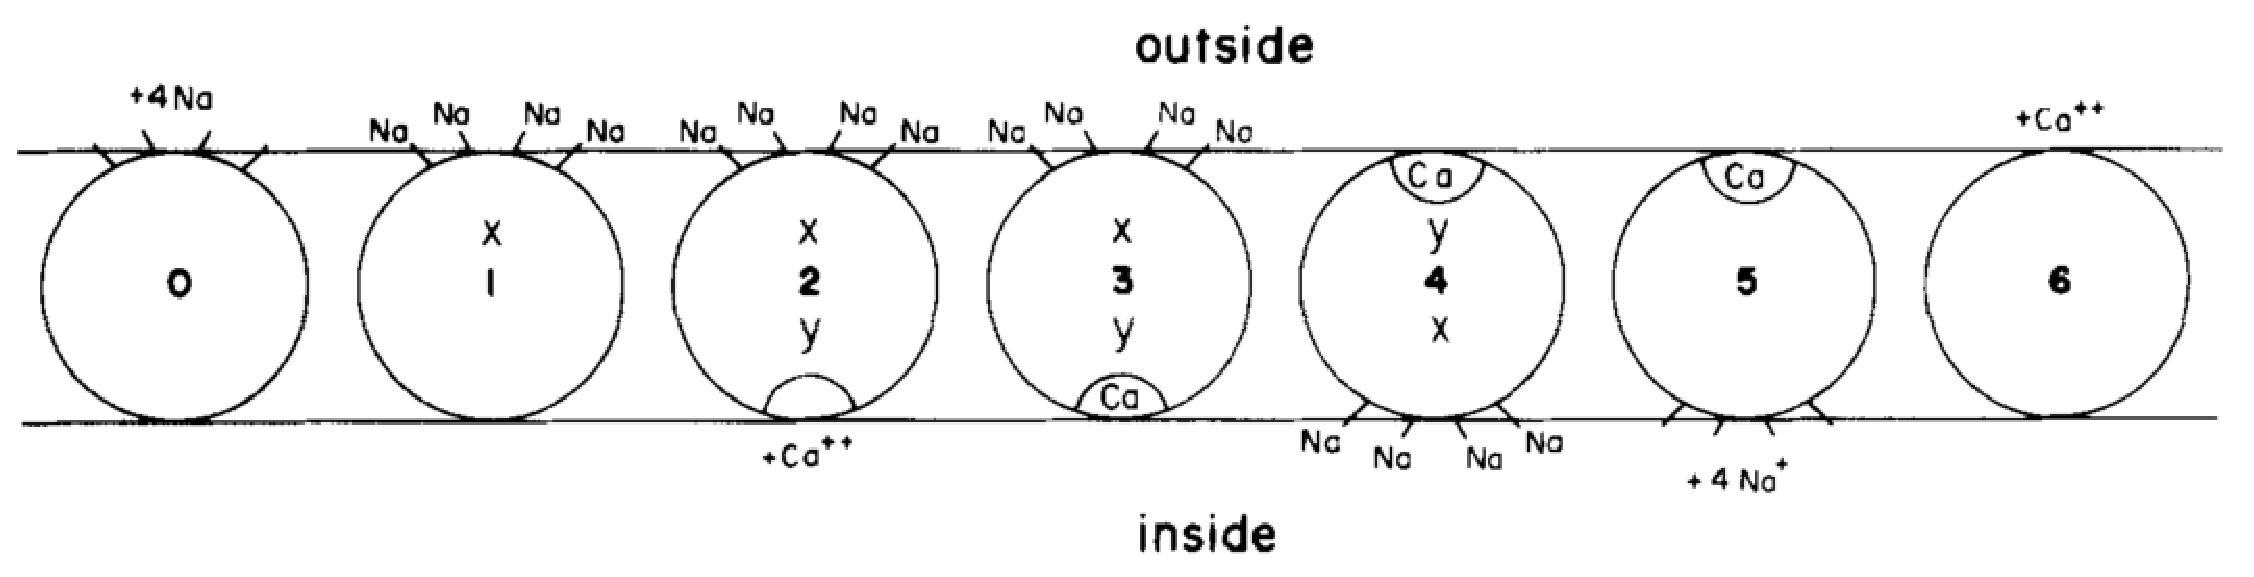
\includegraphics[height=3cm,
    angle=0]{./images/Mullins_NaCa.eps}}
\caption{Sequence of Na/Ca exchange}
\label{fig:Mullins_NaCa}
\end{figure}

The reaction chain for the carrier, read from the lower left corner is
given in Fig.~\ref{fig:Mullins_kinetics}.  Here, X is the $\Na$
binding site, and Y is the $\Ca$ binding site.  The translocation step
$k_7,k_8$ allows totally loaded/unloaded carrier to change $\Na$
binding site on either side of the membrane. This setting is the
feature that emulates ``reverse mode'' of the Na/Ca exchanger. 
\begin{figure}[hbt]
  \centerline{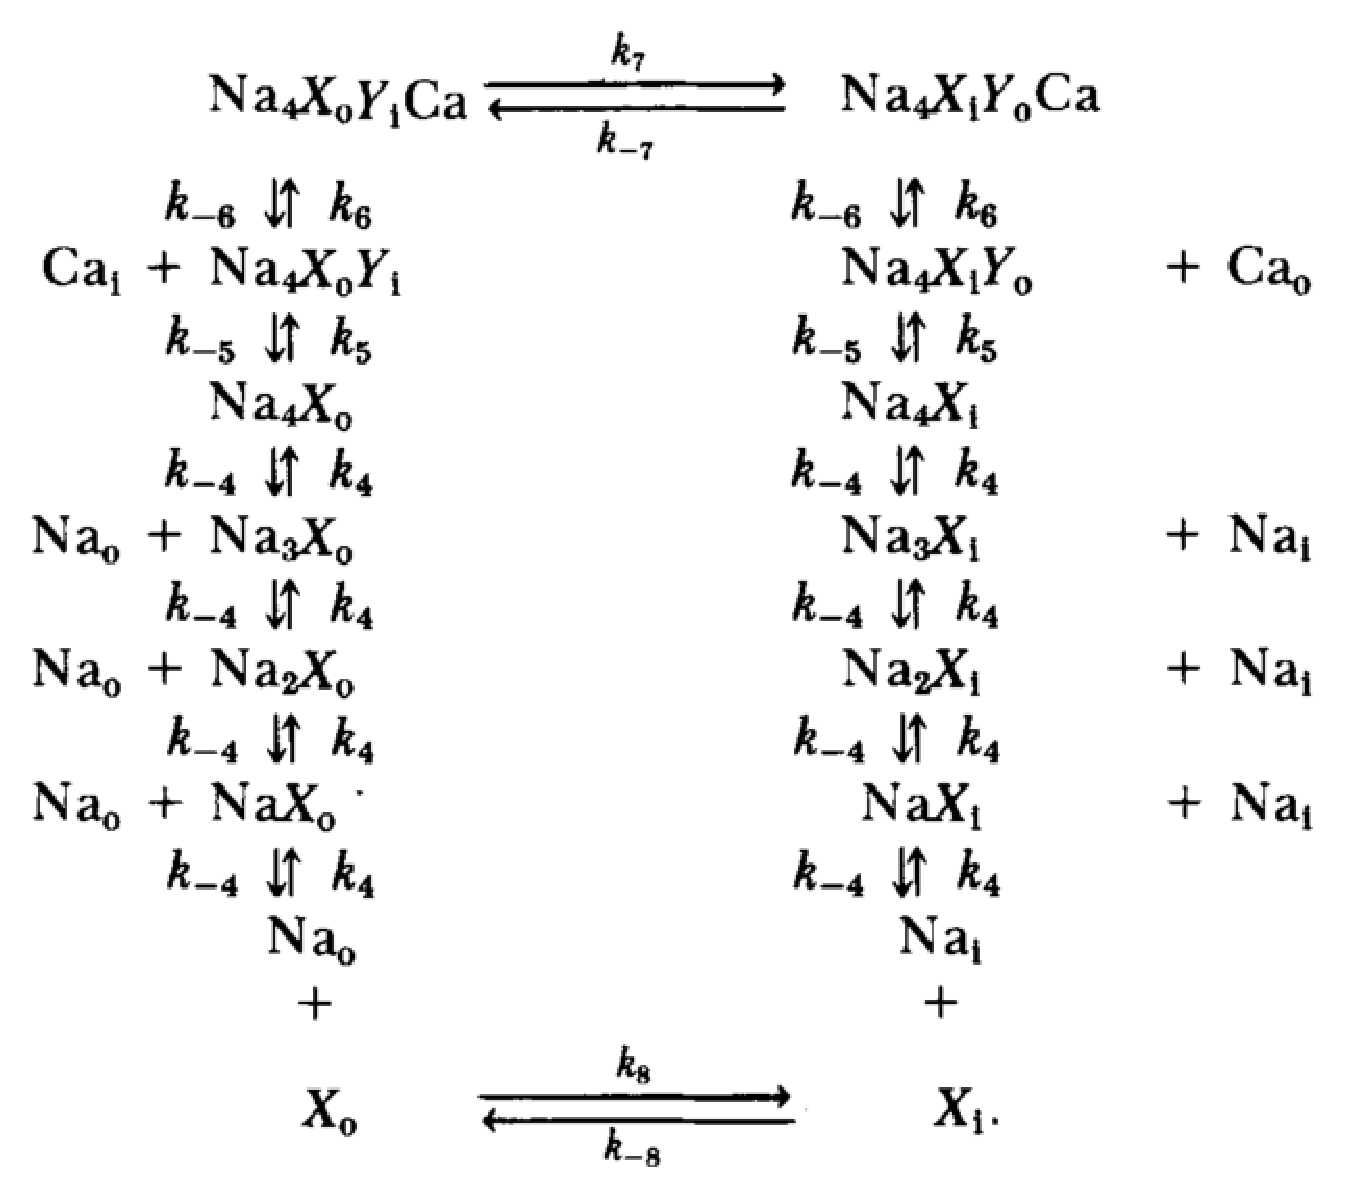
\includegraphics[height=7cm,
    angle=0]{./images/Mullins_kinetics.eps}}
  \caption{Reaction chains of the Na/Ca carrier}
\label{fig:Mullins_kinetics}
\end{figure}

\begin{framed}
  The carrier with less than 4 Na is a poisoned carrier in the sense
  that it cannot carry $\Ca$. Also, the carrier compound $\ce{Na4X_o},
  \ce{Na4X_i}$ are non-mobile forms of the carrier in the absence of
  $\Ca$ binding (e.g. in the absence of $[\Ca]$). The translocating
  forms are $\ce{Na4X_oY_iCa}$ and $\ce{Na4X_iY_oCa}$.
  
  If there is no membrane potential, the two translocating loaded
  carriers will move with equal velocities. With a membrane potential,
  the inward movement is favored by the membrane field.

\end{framed}

For any equilibrium constant of $\Na$ binding to the carrier, there
will be a fraction of population of carriers with less than 4 Na bound
and a fraction with 4 Na bound: $\ce{Na4X_o}, \ce{Na4X_i}$, which
depends on $[\Na]_i$ and $[\Na]_o$. 
\begin{equation}
  \label{eq:1163}
  \ce{[X]_T = [X] + [NaX] + [Na2X] + [Na3X] + [Na4X]}
\end{equation}
To investigate the kinetic scheme above, for simplicity, we can assume
in the absence of $[\Ca]$, $\Na$ is on the outer side only and
$[\ce{Na4X}]$ is equal to $[\ce{Na4XY}]$, so only the first 4
reactions of the left branch are examined.
  \begin{equation}
    \label{eq:1165}
    \begin{split}
      \ce{Na_o + X <=>[K] NaX} \\
      \ce{Na_o + NaX <=>[K] Na2X}  \\
      ... \\
      \ce{Na_o + Na3X <=>[K] Na4X}  \\
    \end{split}
  \end{equation}
with $K=k^-/k^+$ is the equilibrium constant, then 
\begin{equation}
  \label{eq:1166}
  \begin{split}
    [\na]_o[\ce{X}] = K[\NaX] \\
    [\na]_o[\NaX] = K[\ce{Na2X}] \\
  \end{split}
\end{equation}
or (with $j=K/[\na]_o$) \textcolor{red}{Need to reread the paper to
  understand this part}
\begin{equation}
  \label{eq:1167}
  \begin{split}
    ?????
  \end{split}
\end{equation}

\begin{figure}[hbt]
  \centerline{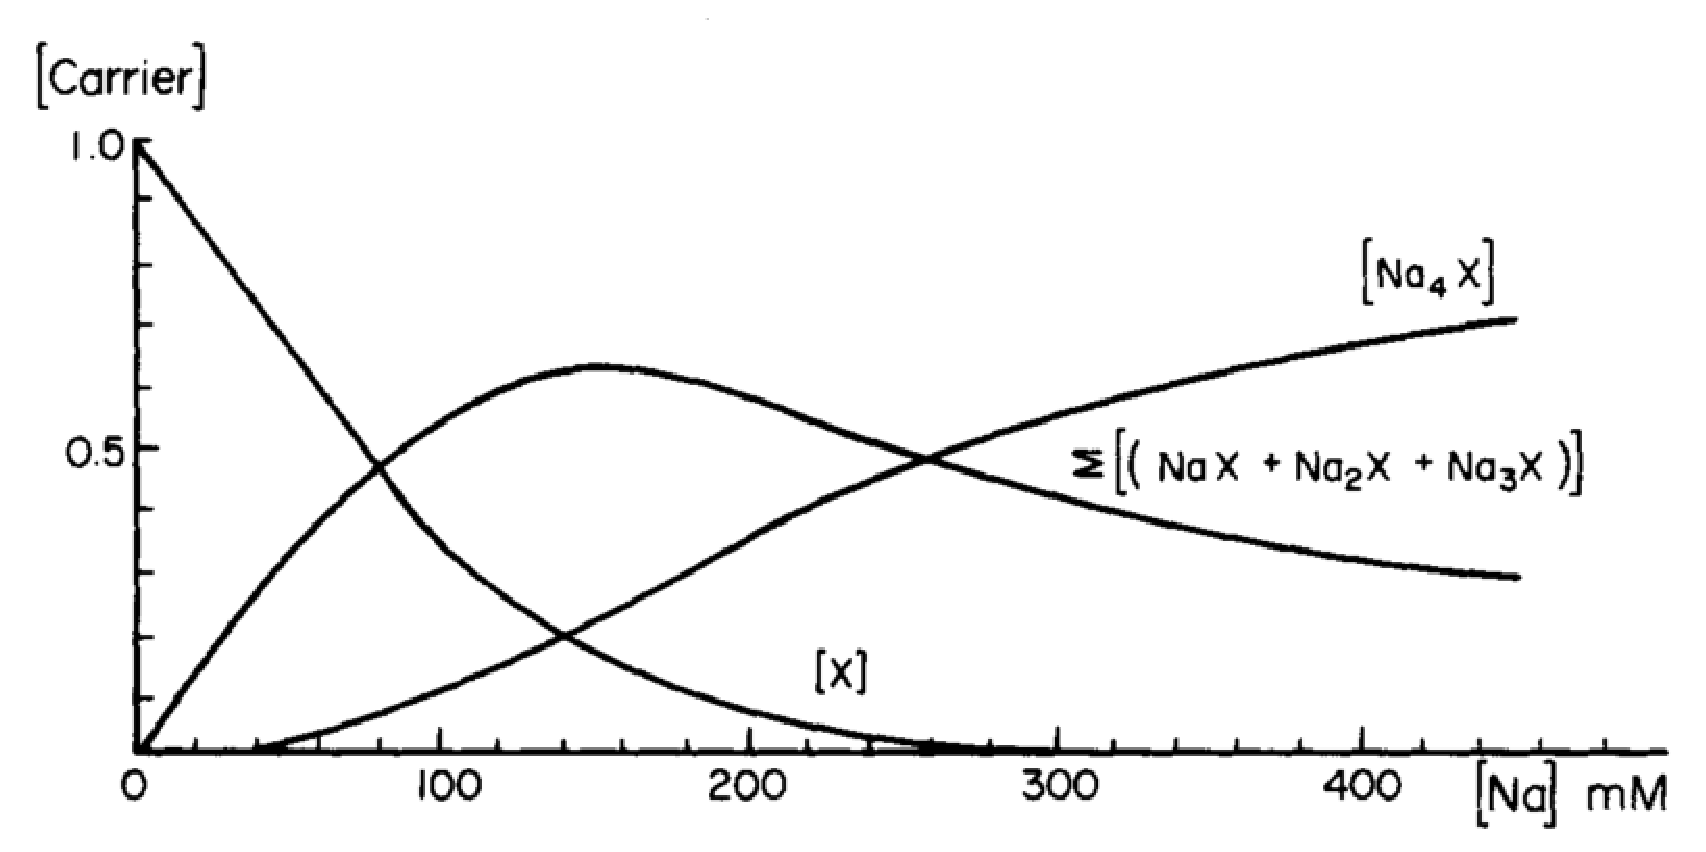
\includegraphics[height=5cm,
    angle=0]{./images/Mullins_carrier.eps}}
\caption{Concentration of Na/Ca carrier in the three forms: [X],
  [$\ce{Na4X}$], and less than 4 Na bound }
\label{fig:Mullins_carrier}
\end{figure}


The kinetics of Na/Ca exchanger must conform to the assumption that
the sole source of energy is the $\Na$ gradient. So, at equilibrium we
have $r\Delta\overline{\mu}_{\na} = \Delta\overline{\mu}_{\ca}$, with $r=4/1$ is
the coupling ration Na/Ca. Then, based on eq. \eqref{eq:1171}, we have
\begin{equation}
  \label{eq:1164}
  \frac{[\Ca]_o}{[\Ca]_i}=\left(\frac{[\Na]_o}{[\Na]_i}\right)^4\exp(-2\frac{V_mF}{RT})
\end{equation}
% The equations to describe the equilibrium state of the scheme above
% are

% As mentioned in Sect.~\ref{sec:introduction-15}, this coupling ratio
% is not accurate, i.e. $n=3$. 

This is the simple form of equation proposed by Mullins which work
well only for small voltage changes and fixed ion concentrations. 
One simply way to model Na/Ca exchanger is using a hyperbolic sine
function of the energy gradient (expressed in mV), as proposed
by~\citep{mullins1977mnc} (Sect.~\ref{sec:ncx-mullins-1977}).
\begin{equation}
  \label{eq:709}
  I_{Na/Ca} =
  k_{Na/Ca}\frac{\exp(\frac{F}{RT}(V_m-E_{Na/Ca})
    -\exp(-\frac{F}{RT}(V_m-E_{Na/Ca}))}{2}
\end{equation}
with
\begin{equation}
  \label{eq:711}
  \begin{split}
    E_{Na/Ca}=\frac{n_{Na/Ca}E_{Na}-2E_{Ca}}{n_{Na/Ca}-2} \\
    E_{Na} = \frac{RT}{F} \ln \frac{[Na]_o}{[Na]_i}\\
    E_{Ca} =  \frac{RT}{z_\ca F} \ln \frac{[\Ca]_o}{[\Ca]_i}
  \end{split}
\end{equation}
with $n_{Na/Ca}$ is the stoichiometry number of the exchanger,
e.g. 3:1 {\it as suggested for cardiac cell}, 4:1
as suggested for squid nerve cell~\citep{mullins1981}, $z_\ca=2$ is
the valence of $\Ca$.  $k_{Na/Ca}=20$ (when $[Na]_i$ in the range
5-10mM, $[\Ca]_i$ in 0.05-0.1$\mu$M).

A more realistic and generalized model was extended
by~\citep{mullins1981} (Sect.\ref{sec:ncx:-mullins-1981}). 

\section{NCX: Mullins (1979)}
\label{sec:ncx:-mullins-1979}

~\citep{mullins1979} use Na:Ca as 4:1 in cardiac fibre. Using
eq.~\eqref{eq:1457}, when Na and Ca electrochemical gradient are
balance, or $2E_\na-E_\ca-V_m=0$, then the $[\Ca]_i$ is given by the
formula
\begin{equation}
  \label{eq:1456}
  [\Ca]_i = \frac{[\Ca]_o([\Na]_i)^4}{([\Na]_o)^4\exp(-2V_mF/(RT))}
\end{equation}

Mullins also shown that $V_m$, $E_\na$, and $E_\ca$ interact to
control the direction of $\Ca$ movement across the sarcolemmal
membrane.



\section{NCX: Mullins (1981)}
\label{sec:ncx:-mullins-1981}

~\citep{mullins1981} describe a more complicated model of NCX.

\section{Kimura et al. (1987) - ventricular cell guinae pig}
\label{sec:NCX_Kimura_1987}

They found that 
\begin{itemize}
  \item NCX current is zero with zero $[\Ca]_i$:
  
  So NCX has an intracellular $\Ca$ binding site which is require to activate
  the exchange of $\Na$ to inside; and $\Ca$ to outside.
  
  \item NCX current is voltage-dependent; with two modes: forward mode and
  reverse mode.

    \item The current below is the sum of inward and outward mode
    
\begin{equation}
\begin{split}
I_\NCX &= k \times \left( 
 [\Na]_i^3 [\Ca]_o \exp \left((n-2).r.F.\Vm/(RT)\right) - \right. \\
 & \left. 
 [\Na]_o^3 [\Ca]_i \exp \left(-(n-2).(1-r).F.\Vm/(RT)\right)
\right)
\end{split}
\end{equation}
with $k$ is scaling factor (unit $\muA$.mM$^{-4}$.cm$^{-2}$) as the factor
controlling the maximum exchange current.

NOTE: It produces an outward current with low $[\Ca]_i$ (i.e.
resting state), and inward current with high $[\Ca]_i$ (i.e. Calcium is being
extruded).

  \item The current shows an exponential function of $\Vm$; yet
  it deviates (as if it saturates) at the potential far away from the reversial
  potential $E_\NaCa$.
  
  \item The coupling ratio (Sect.\ref{sec:NCX-stoichiometry}) that better fit
  the data was chosen as 3Na :  1Ca.

So, 
\begin{verbatim}
ICa = -2 * INCX.
\end{verbatim}
    
    \item Temperature-dependency: Q10 was 3.6$\pm$0.4 at 0mV and 4.0$\pm$ 0.9 at
    50mV in the range between 21 and 36$^\circ$C.
    
    \item Assuming maximum activity of NCX during plateau phase of AP; using
    $[\Ca]_{ER}=1$mM; and activity coefficient 0.33;
    the $[\Ca]_i$ is expected to increase to 3 $\muM$ during an AP.
    Incorporating this value into the $I_\NCX$ equation; and assuming
    140mM $[\Na]_o$; 10 mM $[\Na]_i$; 2mM $[\Ca]_o$; the peak current
    
    $I_{\NCX,\max} = -0.5 \muA/\muF$ is obtained at +10mV of the plateau
    potential. This current corresponds to the $\Ca$ efflux of 50
    $\mu.$mol/(litre.sec); assuming the cardiac myocyte volume 20 pL. 
    
    With this rate, it takes 200ms to expel 10 $\muM$ $[\Ca]_i$ entered through
    the $\Ca$ channels; which is roughly estiamted by Fabiato et al. (1984).
   
   \item At rest: $[\Ca]_i = 270$ nM (guinea-pig ventricle, Coray and McGuigan,
   1981); then the $I_\NCX$ is 
   
   $I_\NCX = -0.035 \muA/\muF$ (or 3.6 $\mu$mol/(Litre.sec)) to flow at resting
   potential, i.e. inward current or reverse mode.

\end{itemize}

The I-V relationship of $[\Ca]_o-$induced and $[\Na]_o$-induced current follows
exponential voltage dependent. Using Eyring rate theory
(Sect.\ref{sec:eyring-rate-theory}).
\begin{equation}
I = a \exp \left(  r F \Vm / (RT) \right)
\end{equation}
with $a$ is scaling factor (determine the magnitude of the current),
$r$ is partition parameter (used in rate theory, represents the
position of the energy barrier in electrical field, which indicates the steepness of
the voltage dependence of the current - Sect.\ref{sec:constant-field-theory}).
\begin{itemize}
  \item $a = 1 - 2	 \muA/\muF$; or equivalently $a = 1-2 \muA/$cm$^2$.
  
NOTE: So the current density is in unit of $\muA/\muF$. However, we can convert
to per unit area using $\Cm=1\muF/$cm$^2$; or 0.01 pF/$\mum^2$.
  
  \item $r = 0.35$ (for $\Ca$-induced outward current)
\end{itemize}
At very positive or negative potentials, the current magnitude became smaller than
expected from an exponential relation.


The outward current magnitude showed a sigmoidal dependence upon the
external Ca2+ concentration with a half-maximum concentration $K_m = 1.38$ mM,
and Hill coefficient of 0.9$\pm$ 0.2.


The outward current magnitude showed a sigmoidal dependence upon the
external Na+ concentration with a half-maximum concentration $K_m = 87.5\pm
10.7$ mM, and Hill coefficient of 2.9$\pm$ 0.4.



If we tentatively assume that k is constant at different external Ca2+ of 1 mM
and 0.1 mM, and the fitted value is  
$k = 2.07 \times 10^{-5}$ ($\muA/($mM$^4$.cm$^2$)) and $r=0.38$; and $E_\NaCa$
is -95.7 mV.

If we use 2.0 mM $[\Ca]_o$, $k=6.28\pm 3.57 \times 10^{-5}$
($\muA/$mM$^4$.$\mu F$) and $E_\NaCa = -100\pm 8$ (mV) (which should be -119 mV
from experimental data).


\section{Gabbiani-Midtgaard-Knopfel (1994)}
\label{sec:NCX-Gabbiani-1994}

The NCX current is modeled based on 3:1 coupling ratio, and
formula of Kimura et al., 1987 (Sect.\ref{sec:NCX_Kimura_1987}).

\begin{equation}
I_\ncx = k_\ncx \left(
[\Ca]_o [\Na]_i^3 \exp ( E_1 \Vm) -
[\Ca]_i [\Na]_o^3 \exp ( - E_2 \Vm)   
\right)
\end{equation}

NOTE: $E_1 = (n-2).r.F/(RT)$; $E_2=(n-2)(1-r)F/(RT)$

with $E_1 = 0.013$ (1/mV); $E_2 = 0.026 $ (1/mV);
$[\Ca]_o = 2$(mM); $[\Na]_o = 152$ (mM); and 
$[\Na]_i = 9$ (mM). The capacity of the exchanger
$k_\ncx = 4.667\times 10^{-4}$ ($\muA$.mM$^{-4}$.cm$^{-2}$) which is 10x higher
than that used in Kimura et al. (1987).

NOTE: The current caused by passing $\Ca$ is 
$I_\ca = -2 I_\ncx$.

\section{Fontana, Blaustein (1995) - rat brain at presynaptic side}
\label{sec:NCX-Fontana-Blaustein-1995}

The $\Ca$ uptake ($J$) is fitted using Hill equation
\begin{equation}
J = J_\max \times \frac{[\Na]_i^{n_H}}{ ([\Na]_i + K_{\na(i)})^{n_H} }
\end{equation}
with $n_H$ is the Hill's coefficients; and $K_{\na(i)}$ is the apparent
concentration of $[\Na]_i$ to induce half-maximal activation of$\Ca$ influx. 
The unit: $J, J_\max$ (pmol (mg protein)$^{-1}$.s$^{-1}$); 
$[\Ca]_o; K_{\na(i)}$ (mM).

The $\Ca$ flux via NCX is modeled as
\begin{equation}
J_\NCX = \bar{J_\NCX} \times A \times B
\end{equation}
with $\bar{J}_\NCX$ is calculated apparent maximal calcium influx at saturating
$[\Ca]_o$; and saturating $[\ce{M^+}]_o$ (total alkali metal ion concentration)
- in the absence of inhibition by $\Na$.

The two factors
\begin{enumerate}
  \item inhibition by $[\Na]_o$: non-competitive inhibition by the co-operative
  action of two $\Na$ ions, i.e. $n_\text{Hill}=1.9-2.0$.
  
  Hill plots for data using $[\Na]_o$ from 10-125 mM yields Hill coefficients of
  1.9-2.0. The implecation is that two extracellular ions act co-operatively to
  inhibit the uptake of $\Ca$.

  
\begin{equation}
B = \frac{1}{1 + \left( \frac{[\Na]_o}{K_{\na}} \right)^2}
\end{equation}
and concentration of $[\Na]_o$ required for half-maximal inhibition of the $\Ca$
influx ($K_{\na}=65$mM).



  \item activation process by the two substrates $\Ca$ and $\ce{M^+}$
  
\begin{equation}
A = \left( \frac{[\Ca]_o \times [\ce{M^+}]}{ K_{\ca(o)} \times K_{\ce{M}} +
     ([\ce{M^+}] \times K_{\ce{M}}) + [\Ca]_o \times [\ce{M^+}]_o }
\right)
\end{equation}
with concentration at half-maximal activation for $[\Ca]_o$ is $K_{\ca(o)}=0.23$
(mM)

\end{enumerate}

The maximal $\Ca$ flux via NCX is 
\begin{equation}
J_\max = 1530 \qquad \text {1530 pmol (mg. protein)$^{-1}$.s$^{-1}$}
\end{equation}




\section{Weber et al. (2001)}
\label{sec:weber-et-al}

~\citep{weber2001} blocked any contribution of SR to $\Ca$ handling;
using drugs to block unwanted sarcolemmal currents (L-type by 20$\mu$M
nifedipine, Ca-activated $\Cl$ current by 30$\mu$M niflumic acid,
Na/K-ATPase by 4$\mu$M N-acetylstrophanthidin). Though $I_\CaT$ was
not blocked, they has not been observed in ferret ventricular
myocyte. If they do, using $V_m=+100$mV, they would only contribute a
negligible Ca influx (since $E_{rest,\ca}\sim
+100$mV)~\citep{satin2000}.

They shown that allosteric $\Ca$ dependent activation of $I_\ncx$
occurs in ferret myocytes and mouse myocytes overexpressing dog
NCX1. The regulation do not occur in WT mouse myocytes, which is
contrast to the results of ~\citep{maxwell1999}. This was explained by
either
\begin{itemize}
\item condition-dependent
\item species differences in amino acid sequence within NCX1. Though
  the sequences are 99\% identical between mouse and dog; a difference
  does occur within the 680-685 region.
\end{itemize}
Amino acids 680-685 are important for $\Ca$ regulation as the
regulation do not occur in mouse overexpressing canine NCX1 lacking
this region.
\textcolor{red}{In summary, the allosteric $\Ca$ regulation should
  only be considered in canine/dog model; but not in mouse models}.

$I_\ncx$ was represented as the product of an electrochemical ($\Delta
E$) and allosteric factor (Allo).

Assumptions:
\begin{enumerate}
\item $\Ca$ activation is an instantaneous process since it's
  impossible to distinguish the spatial and temporal $[\Ca]_i$
  heterogeneous from activation kinetics. 
\end{enumerate}


\section{NCX (reverse mode) - Larbig et al. (2010)}
\label{sec:ncx-reverse-mode}

It's widely accepted that $\ca$ influx is the main trigger for EC
coupling, and NCX is the dominant $\ca$ efflux mechanism~\citep{}.
Pioneer work of~\citep{Leblanc1990} has shown that
\textcolor{red}{NCX can operate in reverse mode at which it pumps
  $\ca$ inside cytoplasm},
which may synergistically combine with LCC current to triggering EC
coupling. Conditions that favour reverse NCX include (1) positive
$V_m$, (2) increase intracellular $[\Na]$ which may exist in early
phase of AP. However, there are studies that shown different
conclusion~\citep{Bouchard1993, Sipido1997}.
\begin{itemize}
\item some studies found NCX and LCC act synergistically to provide
  trigger $\ca$ in CICR. Particularly, the block of $\Na$ channels
  using TTX (tetrodotoxin) showed a decrease in $[\ca]_i$ transient
  magnitude in guinea pig cardiac myocytes.
\item some unable to detect a significant role of reverse NCX to $\ca$
  influx. ~\citep{Sham1992} showed that NCX doesn't activate fast
  enough to have a significant role in the triggering of SR $\ca$
  release.
\end{itemize}

Now, with the available of NCX KO mice, ~\citep{Larbig2010} showed
that $I_\Na$ enhances $\ca$ transient in WT, a feature that is absent
in NCX KO cardiomyocytes. It's believed there is not significant
difference between SR $\ca$ content between WT and NCX KO
myocytes. Thus, this strongly suggests the hypothesis that reverse NCX
triggered by $I_\Na$ during AP upstroke contribute to $\ca$ influx.
\textcolor{red}{They proposed that a non-linear combination of NCX
  current and LCC current results in a more extensive activation of
  RyRs and LCC openings}.

\subsection{Experiments}
\label{sec:experiments}

To inactivate the $I_\Na$ (avoid abrupt rise of $[\Na]_i$), they tried
two approaches:
\begin{itemize}
\item $\Na$ channel blockers TTX
\item gradually depolarize the $V_m$ from -75mV to -45mV using ramp
  prepulse of 1.3s, then hold $V_m=-45$mV for 20ms, followed by a
  brief repolarization -75mV for 2ms before applying the AP clamp
  $V_m=0$mV.

  They vary the ramp prepulse (0.6s - 1.8s), and using -40mV instead
  of -45mV, and it doesn't affect $I_\ca$ kinetics; yet it may
  increase cytoplasmic $[\ca]$ at $V_m=-40$mV. This can be explained
  by reverse NCX, as it doesn't occur in NCX NK myocyte. So, they only
  use -45mV for their experiment. 
\end{itemize}

\subsection{Results}
\label{sec:results}

The inactivation of $I_\Na$ decreases $\ca$ transient amplitude
$51.1\pm4.6\%$ ($P<0.001,n=14$), and reduce SR $\ca$ release by
$53.0\pm 4.6\%$ ($P<0.001,n=14$). 

The effect is larger than observed in~\citep{Leblanc1990}, so it may
be species dependent. The null hypothesis that this effect becomes
more prominent in myocytes of NCX overexpression was rejected
(P=0.07).

